\documentclass[12pt]{article}
\usepackage[top=30truemm, bottom=30truemm]{geometry}

%draftの場合[dvipdfmx]を[draft]
\usepackage[dvipdfmx]{graphicx}
\usepackage{newtxtext}
\usepackage{layout}
\usepackage{lineno}

\usepackage{url}
\usepackage{float}
\usepackage{array}
\usepackage{subcaption}
\usepackage{setspace} 
\setstretch{2}
\usepackage{makeidx}
%bibliographyに必要なパッケージ natbibzip内
%https://ja.sharelatex.com/learn/Bibliography_management_with_natbib
\usepackage{natbib}
\usepackage{lscape}
\usepackage[dvipdfmx]{color}
\usepackage[dvipdfmx]{hyperref}
\usepackage{pxjahyper} %%hyperref読み込みの直後に
\usepackage[toc,title,page]{appendix}

\begin{document}
\linenumbers
\begin{abstract}
Studying the physics of experiments using common materials to simulate geological processes frequently provides novel ideas and insight that can be applied to natural phenomena.
In this study, a physical system of a laboratory experiment that is assumed to be mathematically equivalent to volcanic eruption systems and its behaviors and physical processes are investigated.
This study aims to obtain through a laboratory experiment such new insight and ideas that it would be difficult to find directly from field observation and mathematical modeling of volcanic systems.

In this study, the physics of a pipe-chamber eruption experiment was investigated. 
This experiment was inspired by a sugar syrup eruption experiment conducted as an exhibition during an institute open house. 
The experimental system comprised a vertical pipe connected to a gas chamber where a constant gas flux was maintained in the gas chamber and the gas-liquid flow in the pipe.

First, pressure changes in the chamber were investigated. Sawtooth wave-like pressure changes (STW) were observed during the constant gas supply. Similar waveforms have been observed as geodetic signals that are associated with repetitive explosive eruptions and Dome-building eruptions.
Volcanic oscillations have been explained by flow-induced oscillation models that include a coupling between elastic capacitance and variable flow resistance.
Behaviors of these systems have not been studied by laboratory experiments. 
It was shown that the experimental system of this study was mathematically similar to the existing volcanic oscillation models.
The chamber pressure changes and flows in the pipe in the experiment were comparable with magma chamber pressure changes and conduit flows in volcanic systems, regardless of differences in specific scales and flow structures.
In the experiment, periodicity spontaneously varied in either non-periodic, bimodal or trimodal manners, even if the given experimental parameters such as the pipe-chamber geometry and gas influx were constant.
These had not been expected from existing models of volcanic systems. 
Finding such new phenomena is a significance of the lumped parameter model experiment of volcanic systems.
As a result of the flow image analysis, it was concluded that the spontaneous periodicity fluctuations were caused by variations of flow structure in the pipe due to past gas emissions.
I inferred that, in the actual volcanic systems, fall-back of ejected materials, dike collapse, or different depth of magma head could disturb periodicity of an eruption.

Second, acoustic waves were measured at the top of the pipe in association with the chamber pressure oscillations and gas emissions.
The acoustic waveforms were disturbed preceding that the flow structure in the pipe and the chamber pressure periodicity were disturbed.
In general, the acoustic waveforms with the sawtooth wave-like pressure changes in the chamber had two characteristic frequency peaks. The peak frequencies were explained by two different resonance models.
It was shown that the amplitude of the lower frequency band in the acoustic wave had good correlation with the sawtooth wave amplitude in the chamber.
Although the mechanisms of acoustic wave generation in this experiment and those in volcanic systems have not sufficiently linked, this experimental results suggested a possibility to find a correlation between a particular component of infrasound and ground deformation observed in actual volcanic eruptions.

Finally, relationships among ground deformation, infrasound, and video records during 2015 Sakurajima volcanic activity were investigated.
The recurrence interval of sawtooth wave-like ground deformation was by far disturbed compared to the experimental results. It was not successful in finding a relation between successive events that was comparable with the experimental system.
The main finding was that the correlation between the sawtooth wave amplitude of ground deformation and the cumulative energies of small infrasound signals during the individual ash eruption events. It was suggested that the infrasound energy would be a useful parameter for monitoring eruptive volcanic activity.
                
In this study, I have not completed updating volcanic models based on insights and ideas obtained from experiments.
On the other hand, showing the mathematical similarity between the experiment and volcanic eruption systems, finding disturbed periodicity and the correlation between a particular resonance model of infrasound and chamber pressure were important results. 
They were unique outcomes of a model experiment of volcanic systems. 
The obtained relationship between infrasound and ground deformation at Sakurajima was found as a result of reviewing and analyzing the observational data applying insights from the laboratory experiment.
Based on the above results, this experimental system may provide a useful tool for understanding volcanic eruption system.
\end{abstract} 



\newpage
\cleardoublepage


\section{Introduction}\label{ACOintro}
火山が, 20 Hz以下の音波として定義される空振音源であることは, よく知られている.
空振観測は,観測所,監視カメラ, あるいは悪天候,夜間,離島の噴火がない場合でも, 噴火の発生とその方向を検出することできる. 
したがって, 防災の観点からも重要な物理観測量のひとつである.
また, 空振はさまざまな固有周波数と波形を持っている. 
発生メカニズムを考慮すれば, 噴火質量や噴火率などの噴火パラメータを推定することが可能であると期待される.

It is well-established that volcanoes are sources of infrasound, defined as acoustic, or sound, waves below 20 Hz.
Infrasound observations can detect eruption occurrence and its direction even in the absence of observation stations, surveillance cameras, or in the poor weather, nighttime, or eruptions in remote islands.
Therefore, it is one of the important physical observation from the standpoint of disaster prevention.
Also, infrasound signal has various characteristic frequencies and waveforms.
It is expected that it is possible to estimate the eruption parameters, such as eruption mass and rate through infrasound analyses.

本研究では, 実験で測定した音波の解析, 共鳴励起のメカニズムの解明, 同時に記録されたチャンバー圧力と流動様式との対応関係の解明を目指す.
実験の空気振動に関しては, 特に周波数構造に着目し, そのメカニズムを検討した. 

In this study, we aim to analyze the acoustic wave measured in our experiment, identify the mechanism of resonance excitation, and clarify the correspondence with the chamber pressure and flow pattern recorded at the same time. 
Regarding the acoustic wave of the experiment, especially, we paid attention to the frequency structure.


\subsection{Laboratory experiments}\label{AcoinEx}
\cite{Vidal2006a}では, 円筒状のCavity上部に張った石けん膜が, Cavity内部の過剰圧によって割れる際の空気振動を計測した. 
この実験は, 大気泡が火道浅部で破裂すると考えられているストロンボリ式噴火 \citep{Chouet1974, BLACKBURN1976, Vergniolle1996c} での空振発生プロセスを再現していると考えられている \citep{Vidal2010a, Gerst2013a}.
この実験において, 発生する空気振動の周波数構造は, Cavity内の定在波, すなわち, 閉管の気柱共鳴で説明できる. 
一方で, 破裂後, 管の外で計測した空気振動の振幅は, 破裂直前のCavity内の過剰圧には相関せず, 膜の破裂過程に大きく影響される. 
すなわち, キャップの破裂・破壊をともなうような噴火においても, 空振の振幅はキャップの破裂・破壊過程に影響を受ける可能性が示唆される \citep{Vidal2010a}. 
\cite{Sanchez2014}では, 石けん膜の代わりに, Elastic membraneを用いて破裂速度を制御した実験を行った. 
この結果, やはり特徴的な周波数は閉管気柱共鳴で説明できる. 
また, 膜の破裂速度を制御すれば, 破裂前の過剰圧が小さい (この実験では 24 kPa以下) 時に, 破裂前過剰圧と破裂時の空気振動振幅が線形な関係にあることを示した. 

\cite{Vidal2006a} reported an experimental study of the acoustic wave produced by the bursting of a thin soap film, which initially closes an overpressurized cylindrical cavity.
This experiment is believed to reproduce the process of occurrence of infrasound in Strombolian eruption \citep {Chouet1974, BLACKBURN1976, Vergniolle1996c}; bursting of large gas bubbles in the shallow part of the conduit  \citep{Vidal2010a, Gerst2013a}.
In this experiment, the frequency structure of the acoustic pulse can be explained by the standing wave in the cavity, that is, the air column resonance of the closed pipe.
On the other hand, the amplitude of the acoustic wave measured outside the pipe does not correlate with the overpressure in the cavity just before rupture; it is greatly influenced by the rupture process of the membrane.
It was suggested that the amplitude of infrasound might be influenced by the fracture process of the cap even in the eruption accompanying the rupture/destruction of the cap \citep{Vidal2010a}.
In \cite{Sanchez2014}, an experiment was conducted in which the rupturing rate was controlled using an elastic membrane instead of the soap film.
As a result, the characteristic frequency can also be explained by closed air column resonance.
Also, by controlling the rupture rate of the membrane, it was shown that the pre-rupture overpressure and the acoustic pulse amplitude at the time of rupture are in a linear relationship when the overpressure before rupture is small (24 kPa or less in this experiment).

流体内を上昇し, 表面で破裂する気泡によって発生する空気振動も, 室内実験によって調べられている.
\cite{James2004}では, 鉛直パイプ内に満たされたニュートン流体中のガススラグの上昇と破裂過程における空気振動を計測した. 連続的なガススラグの上昇と破裂の際に計測された空気振動の特徴的な周波数は閉管の気柱共鳴で説明できる. 
\cite{Spiel1992}では, 気泡サイズよりも十分に大きな水槽中を上昇する気泡の破裂によって生じる空気振動を計測した. 空気振動の特徴的周波数は気泡破裂時の気泡体積と, 気泡サイズに対して小さい開口面積に由来するヘルムホルツ共鳴であると推定している.
\cite{Divoux2008}では, 非ニュートン流体中を上昇する気泡の破裂にともなう空気振動を計測した. 空気振動の特徴的な周波数は, カスプ状に尖った気泡の形状に依存する共鳴音であると推定している.

The acoustic waves generated by gas bubbles rising in the fluid and bursting on the surface have also been studied by laboratory experiments.
\cite{James2004} measured pressure changes during the rise of the gas slug in the Newtonian fluid filled in the vertical pipe and the acoustic wave in the bursting process.
The characteristic frequency of the acoustic wave measured during the continuous rise of gas slug and rupture was explained by the resonance of closed air column.
\cite{Spiel1992} measured the acoustic wave caused by the bursting of bubbles rising in the water tank, which was sufficiently larger than the bubble size.
The characteristic frequency of the acoustic wave was explained by the Helmholtz resonance as a consequence of the bubble volume acting as a resonator when trapped gas tries to escape through the small hole in the top of the bubble.
\cite{Divoux2008} measured the acoustic wave associated with the bursting of bubbles rising in non-Newtonian fluids.
They estimated that the characteristic frequency of the acoustic wave is a resonance that depends on the cusp-shaped bubble shape.

\subsection{Observation}\label{AcoinObs}
ストロンボリ式噴火では, 低粘性マグマ中を大気泡が上昇し, 表面で破裂すると考えられている. 大気泡の破裂にともない, 継続時間が数秒程度のパルス状空振が発生する.
\cite{Vergniolle1996b} では1992年, ストロンボリ島 (イタリア) において空振観測を行った. この観測では Br\"uel-Kj\ae r社製マイク (Type 4155, 1 Hz - 70 kHz, Type 4165, 4 Hz - 20 kHz) を用いて, 3点の観測点 (東火口から約 250 m地点に 2点, 約 370 m地点に 1点) で, 1 kHzサンプリングで空振を記録した. 
この時期のストロンボリは, 西火口ではマグマを目視でき, 泡の破裂が確認できる. 一方で, 東火口の活動は比較的穏やかであった. 
東火口で発生した爆発の際に観測した空振にともなって, Fig. \ref{Verg19961fig1}aのような波形を観測し, 主要相では約 10 Hz にピークを持つ (Fig. \ref{Verg19961fig1}c). この波形を説明するメカニズムとして, \cite{Vergniolle1996c} では, 気泡破裂前の, 気泡膜振動が提案されている. 
しかし一方で, 近年のレーダー観測を用いた大気泡膨張過程における気泡膜移動速度の直接観測 \citep{Gerst2013a} によれば, 膜の振動は計測されず, 大気泡は空振波形の希薄相が始まる前に破裂しており, 特徴的周波数は膜の破裂後, 表面に取り残された空洞部分の共鳴であると推定している (Fig. \ref{gerst2013f14}).

During Stromboli eruptions, it is thought that the large gas bubbles rise in the low viscous magma and burst on the surface. Infrasound signals with durations of a few seconds or less are observed.
\cite{Vergniolle1996b} made infrasound observations at Stromboli (Italy) in 1992. 
In this observation, set up for the observations consists of microphones (Br\"uel-Kj\ae r Type 4155, 1 Hz - 70 kHz, Type 4165, 4 Hz - 20 kHz), and signals were recorded with 1 kHz sampling at three observation points (two points at about 250 m from the east crater and one at about 370 m).
In April 1992, the lava in the western crater has been observed visually, and bubbles have been observed to break at the surface.
As a mechanism to explain the acoustic pressure waveform, in \cite{Vergniolle1996c}, bubble film vibration before bubble rupture is proposed.
On the other hand, according to direct velocity measurements of the expanding magma shell surface using Doppler radar observation in recent years, oscillations of the intact bubble surface were not measured.
They suggested that generation of the infrasound signal as a result of a dual mechanism: following the initial infrasound signal generation by an expanding bubble shell, it could be explained by a resonating gas slug cavity within the evacuated conduit.

ブルカノ式噴火は島弧の安山岩質火山でしばしば発生し, 単発的・間欠的に爆発が起こる噴火である. 
\cite{Iguchi2008}では, 地震と地盤変動観測の解析から, 火道浅部のプラグが破壊されることによって噴火が発生していると推定している.
2011年桜島昭和火口の噴火を対象とした空振観測では, 空振がふたつの特徴的ピーク周波数 (0.2 - 0.5 Hz と1 - 2 Hz) を持つことが報告されている \citep{yokoo2012bo}. 
前者のピークは昭和火口の噴出口の固有振動数に関係し, 後者は噴火雲のダイナミクスに関係すると考えられている \citep {yokoo2012bo}.
%この観測では白山工業社製マイク (SI102) を用いて, 昭和火口から約 3.3 km東にある黒神観測点において, 200 Hzサンプリングで, 9台のマイクを用いたアレイ観測を行った.
%三次元噴煙計算 \citep{Suzuki2005} によって, 噴出率 10$^6$ kg/s, 噴出速度 133.67 m/s, 温度 1273.15 K, 火口直径 20.37 m の時の噴煙を再現すると, 0.3 - 0.6 Hzあたりにパワーが集中し, 1 - 2 Hz付近のシグナルは含まれない. 
%一方で, 実際の観測値においては, 1 - 2 Hzのシグナルは噴火発生の有無と関係なく観測される. 従って, \cite{yokoo2012bo} では, 0.2 - 0.5 Hzのシグナルは噴煙から放射されており, 1 - 2 Hzの周波数帯のシグナルは, 火口や火道部分がガスや噴煙の通り道となることで固有振動数が強められるのではないかと考えられている. 

Vulcanian eruptions involving strong short-lived (discrete) eruptions and the ejection of volcanic bombs and ash are common for andesitic volcanoes in island-arc areas.
These explosive eruptions is generated by failure of the cap and these phenomena are investigated based on seismic and ground deformation observations \citep{Iguchi2008}.
Results of the 2011 infrasound observations at Sakurajima volcano suggest there are two peaks, around 2 Hz and 0.5 Hz, in the power spectrum of the infrasound. 
The former peak would be related to the eigenfrequency of the vent of Showa crater, and the latter would be related to dynamics of eruption clouds \citep{yokoo2012bo}. 


%微動型の空振はどこまでいれるか?どのような意図でいれるか?

%継続時間が長い, 微動型の空振も報告されているが, 本実験では, チャンバー圧力振動にともなって, パルス的な空気振動が発生しているため, 微動型空振の先行研究は簡潔にまとめる. 
%詳細についてはAppendix (\S \ref{appeaco}) にまとめる.

%チリのビジャリカ火山では, 溶岩湖内マグマの対流と, 表面での気泡破裂が発生している時期に, 0.77 Hz付近にピークを持つモノトニックな空振が報告されている \citep{Ripepe2010b, Goto2011}. 
%\cite{Ripepe2010b}では, 計測されるモノトニックな周波数ピークは気液二相流の重力的な不安定による火口湖表面の振動に起因すると推定した. %Ripepe2010 p4
%一方で, \cite{Goto2011}で撮影したビデオ映像によれば, 火口湖表面での対流や脱ガス活動と, 空振記録との間に明瞭な関係が見られなかったことから, 特徴的周波数は空洞状の火口内気体の体積振動, すなわちヘルムホルツ共鳴であると考えられている. %Goto2011 p.3
%このような空洞状の火口内のヘルムホルツ共鳴と考えられる空振は, キラウェア火山 (ハワイ), ハレマウマウ火口における連続的な脱ガス活動の際にも報告されている \cite{Fee2010c}. 
%この活動で観測された空振には, もう一つ特徴的なピークがあり, 空洞状の火口内の定在波であると推定されている (Fig. \ref{fee2010bfig3}). 

%セントへレンズ山 (アメリカ)では, 2005年3月に, 最大高度が 9 km程度の噴煙柱を形成する噴火の際に, 0.2 Hz付近に周波数ピークを持つような空振を観測した (Fig. \ref{matoza2009f2}). 
%この観測では, MB2000微気圧計 (0.01-17 Hzで平坦な特性)を用いて, 火口から13 km 北西のColdwaterという観測点で, 40 Hzサンプリングで4点空振アレイ (100 m間隔) 観測を行った. 
%この周波数構造は, ジェットノイズの周波数構造と相似的であり, 自己相似的なノイズ (Large-scale turbulence) 生成メカニズムの存在が示唆される \citep{Matoza2009a}.

%エクアドルのトゥングラワ火山 \citep{Fee2010} では, 2006年7月14-15日 (UTC) の噴火で, 火口直上に噴煙柱を形成する継続的なジェット噴出の際に, 0.25 Hz付近と 1 Hz付近に幅の広い2つのピークを持ち, その間にノッチを持つような周波数構造を持つ空振を記録した (Fig. \ref{fee2010afig9}点線). 一方で, 7月15日 2:45 (UTC) ごろに発生した Pyrocclastic density current (PDC) にともなって記録された空振では, 0.25 Hzのみにピークを持つ周波数構造であった. 1 Hz付近のピークは, 噴煙柱を形成するような噴火において見られる特徴的ピークであることから, 自己相似的なノイズ (Large-scale turbulence) 生成メカニズムの存在が示唆される \citep{Matoza2009a}. また, 0.25 Hzのピークは, PDC 発生時においても見られたことから, 流れと火口壁との相互作用に起因すると考えられている.
%噴煙柱を形成するような噴火では 1 Hzのピークが見えるため, 1 Hzのピークはジェットノイズに関係し, 0.25 Hzのピーク固体粒子間の相互作用に由来するのではないかと考えられているが \citep{Matoza2009a}, 定量的な議論はなされていない.


%基本周波数と, その倍音成分を持つハーモニックな微動型空振も多くの火山で報告されている. サンガイ山 (Sangay, エクアドル)では, 1998年4月の観測で, Chugging発生時に基本周波数が約1 Hzのハーモニックな微動型空振を計測している \citep{Johnson2000}. Chugging発生と同期したハーモニックな微動型空振は, アレナル山 (Arenal, コスタリカ, 1997年) \citep{Hagerty2000}, カリムスキー山(Karymsky, ロシア, 1997-98年) \citep{Johnson2000}, レベンタドル山 (Reventador, エクアドル, 2005年) \citep{Lees2008}, 桜島 (2017年) \citep{sakai1996, iguchi2018} でも報告されている.


\clearpage
\subsection{Infrasound-derived eruption parameters}\label{AcointPara}

火山活動にともなう空振記録の解析と, そのほかの物理観測量とを用いることで, 噴火の物理過程や, パラメータを推定する試みがなされている. 
爆発的噴火にともなうパルス状の空振に関しては, 空振のソースが単純なモノポールソースであると仮定し \citep{Lighthill1978}, 積算体積を推定する手法が提案されている \citep{Johnson2003}. この手法を用いて, 空振から見積もった積算体積と, そのほかの観測量とか比較されている.

Attempts have been made to estimate the physical processes and parameters of the eruption by infrasound observations and combining other physical observations.
For explosive eruptions, a simple monopole source is assumed \citep{Lighthill1978} and a method for estimating the cumulative volume has been proposed \citep{Johnson2003}.
Using this method, infrasound-derived gas volume has been compared with other observation parameters.

\cite{Dalton2010}では、Gas-richな小規模噴火における空振から推定した噴出体積と, UVカメラによって得られたガス質量とがおおむね比例関係にあることを示した.
また, 多くの火山灰放出をともなう Ash-richな火山活動, とくに爆発的噴火に関して, \cite{Fee2017a}では, 桜島の爆発空振から推定した噴出量, 火山灰降下量, ガス観測から推定した噴出量とを比較した. この結果, 空振から推定した噴出量と, 火山灰の堆積分布から推定した噴出量とは, 一桁程度のばらつきをもって比例関係があると主張している.
\cite{Yamada2018b}では, 空振波形の積分から推定した噴出体積 ($V_{inf}$)と, 時定数の短い噴火にともなう噴煙をサーマルに近似することで推定した噴煙体積 ($V_{b}$) の関係を調べた. この結果, $V_{b}/V_{inf}=16$という関係を得た. 
空振から推定した体積は, 爆発の初動段階で火口付近で押しのけられた体積を反映していると考えている. 

\cite{Dalton2010} showed that infrasound-derived gas volume during small-scale gas-rich eruptions was consistent with the gas masses derived by UV cameras.
Particularly for ash-rich eruptions, \cite{Fee2017a} attempted to validate the infrasound-derived eruption masses by comparing them to independently derived, ground-based eruption mass estimates constrained through ash sampling and remotely sensed measurements of SO$_2$. They contended that the infrasound and ground-based eruption masses are similar within less than an order of magnitude.
The relationship between infrasound-derived volume ($V_{inf}$) and the buoyancy-derived volume ($V_{b}$) based on the one-dimensional model for the rise of a discrete thermal was examined by \cite{Yamada2018b} and they obtained a representative ratio of $V_{b}/V_{inf}$ of 16. 
They contended that $V_{inf}$ corresponds to the volume that would be displaced by the emerging jet.

しかし一方で, Gas-rich, Ash-richな噴火それぞれに, 単純にモノポールソースを仮定して良いかは自明ではない. \cite{DelleDonne2016} では, イタリア, ストロンボリ火山における空振記録に対して, 初期の空振パルス波形だけではなく, その後の後続波まで含めた波形を用いて推定した噴出量と, UVカメラを用いて推定した噴出量とが, Ash-rich, Gas-richな噴火共に, 良い相関を持つことを示した. 
\cite{Ichihara2016a}では, 新燃岳 2011年噴火の際に観測された3回のサブプリニー式イベントにおいて, 地盤変動から推定した噴出率 ($\dot{V}_m$) と, 地震・空振パワー (SET, AET) の関係を調べた. 
この結果, 準定常的サブプリニーイベント発生時には, すべてのペアの推定値が, 線形関係にあることを示し, 定常的な噴火の際の空振が, 破砕面での連続的な爆発によって励起されていると推定している. 
この結果からは, ある特定のイベントにおける空振に着目すれば, 空振と噴出率・量の対応関係を見出すことができる可能性が示唆される.

It is not obvious whether we can simply assume a monopole source for each of the Gas-rich and Ash-rich eruptions.
\cite{DelleDonne2016} showed that infrasound-derived gas masses estimated not simply by the initial pressure but rather the full infrasonic waveform are consistent with the gas masses derived by UV cameras for both ash-rich and gas-rich eruptions recorded at Stromboli volcano, Italy.
Pairwise power law relationships between seismic eruption tremor power (SET), acoustic eruption tremor
power (AET), and magma discharge rate ($\dot{V}_m$) based on ground deformation were investigated for eruption tremor recorded during three sub-Plinian events during the 2011 eruption sequence of Shinmoe-dake, Japan \citep{Ichihara2016a}. 
Linear relationships are observed between all pairs of parameters during the quasi-stable or slowly growing stages of the sub-Plinian events. 
A possible explanation is that both SET and AET are generated by successive explosions at the fragmentation surface in the conduit. 
Focusing on the specific signal of infrasound at a certain event, it is suggested from these result that it is possible to find a correspondence relation between infrasound and magma discharge mass and/or rate.

\clearpage \newpage
\subsection{Methods}\label{ACOresult}
実験装置及び実験手法は \cite{kanno2018} で行なった実験と同じである. 
本章では液スラグ膜の破裂によって発生し, パイプ上端のマイクで捉えた空気振動に着目する. 
特に, 空気振動と, 前章で議論したチャンバー圧力振動との関係に主眼を置く.  

Based on the laboratory experiments carried out by \cite{kanno2018}, we investigate the acoustic wave produced by overpressure release by each burst cycles of layered liquid slug structure. 
In particular, relationships between chamber pressure and acoustic wave are examined.

実験装置の概要を以下に示す. 

The experimental system comprised a chamber and pipe, where a constant gas flux was maintained in the chamber, and the gas-liquid flow in the pipe.
Vc is maintained at a constant value during each experimental run. 
We used sugar syrup diluted in distilled water as the liquid phase. 
The liquid behaved as a Newtonian fluid and adjusted it to 1 Pas at the experimental temperature of 25 °C. 
Injected gas flowed through the pipe and forced the liquid residing in the pipe upward, resulting in gas-liquid flow within the pipe.
A pressure sensor (KISTLER 701Awith a 5011A charge amplifier) was installed to measure pressure changes in the chamber, and a microphone (Br\"uel-Kj\ae r 4193+2669L with a Nexus 2690 signal conditioner) was mounted to the top of the pipe. Data were sampled at 10 kHz using a PC- based data acquisition system (DEWETRON DEWE-211). A high-speed black-and-white camera (Photron FASTCAM Mini) was synchronized with the data acquisition PC and was focused on the lowermost 200 mm of the pipe, where gas-liquid flow occurred. The field of view was illuminated by a flat backlight source. We used a pale-color syrup to improve the visibility of the liquid phase against the gas phase and the pipe. Dark areas were thus shaded according to the thickness of the liquid across the pipe.

Under relatively large Qin and Vc, unimodal STW is observed, which consists of gradual pressure increase during slug flow and abrupt pressure drop at the slug-to-annular flow transition. Under small Qin and Vc, only slug flow with small pressure fluctuation is observed, referred to as small fluctuation. With a far larger Qin, the periodicity of STW is lost and we observe large surface disturbances on downward film flow causing slug reconstruction at varying locations along the pipe. It is referred to as disturbed STW.

\clearpage \newpage
\subsection{Results}\label{ACOresult}
\subsubsection{Outline of measured acoustic wave}
Unimodal STW が発生している時 ($Q_\mathrm{in}=$ 0.6 cm$^3$/s, $V_\mathrm{c}=$ 122 cm$^3$) のチャンバー圧力と空振記録の時間変化をFig. \ref{MonoPAtime}に示す. 
振幅の大きな (> 10 Pa) 空気振動は, STWの急激な圧力減少と同期している.
空気振動の代表的な波形とスペクトルを Fig. \ref{Monowaveform}に示す. 
実験において, 圧力急減少の有無を問わずに, 空気振動パルスの最大振幅が 1 Pa以上になるようなパルスをトリガし, 縦軸が周波数, 横軸がパルスイベントになるように並べた図を Fig. \ref{Monopspec}に示す. 
イベントは, 20 Hz付近のピークの大きさでソートしてある. 
この結果によれば, 低周波帯 ($\sim$ 20 Hz) にピークを持つ波形は, 230 - 270 Hz付近にもピークを持つ. 
一方で, 低周波帯にピークを持たないパルスは, 180 - 200 Hz付近に明瞭なピークをもち, 270 Hz付近に小さいピークを持つ. 
この実験条件で発生する空振のうち, 半数程度は低周波帯にピークを持たない空振であった. 
以下, 低周波帯 (< 50 Hz) と高周波帯 (> 150 Hz) にピークを持つパルスを低周波パルス, 高周波帯 (> 150 Hz) のみにピークを持つパルスを高周波パルスと呼ぶ. 

For unimodal STW ($Q_\mathrm{in}=$ 0.6 cm$^3$/s, $V_\mathrm{c}=$ 122 cm$^3$), pressure change in the chamber and the microphone at the pipe exit is shown in Fig. \ref{MonoPAtime}.
Acoustic pulses with large amplitude (> 10 Pa) were coincident with an abrupt pressure drop in the chamber.
Representative acoustic waveform and its spectrum are shown in Fig. \ref{Monowaveform}.
In the experiment, acoustic pulses were triggered by its amplitude (> 10 Pa), regardless of chamber pressure drop occurred or not. 
An event-spectrum representation is shown in Fig. \ref{Monopspec}. 
According to this result, the acoustic waveforms having a peak in the low-frequency band ($\sim$ 20 Hz) also had a peak in the vicinity of 230 - 270 Hz.
On the other hand, acoustic waveforms with no peak in the low-frequency band had clear peaks around 180 - 200 Hz and small peaks around 270 Hz.
Among the acoustic waveforms generated under unimodal STW conditions, about half of them did not have a peak in the low-frequency band.
Hereinafter, a pulse having a peak both in a low-frequency band (<50 Hz) and a high-frequency band (> 150 Hz) is referred to as a low-frequency pulse, and a pulse having a peak only in a high-frequency band (> 150 Hz) is referred to as a high-frequency pulse.

Small fluctuation 発生時, すなわち, 連続的なスラグ流が計測される際のチャンバー圧力と空振記録を Fig. \ref{FlctPAtime} に示す.  
STW発生時と比較して, チャンバー圧力変動との対応は不明瞭であるが, 概ね緩やかな圧力減少と空気振動の発生が対応している. 代表的な波形を Fig. \ref{Flctwaveform} に示す. 
パルスの振幅はSTW発生時と比べて小さく, 低周波帯にピークがみられない. 
Fig. \ref{Flctpspec} に Fig. \ref{Monopspec}と対応した図を示す. 
この実験条件では, 180 - 200 Hz程度に基本周波数を持つ振動が発生している. 
波形及び周波数ピークの特徴から, STW発生時の高周波パルス (Fig. \ref{Monowaveform}a-c) と同じ性質を持つ. 

Fig. \ref{FlctPAtime} shows chamber pressure and acoustic wave under the small fluctuation conditions, that is when continuous slug flow was measured.
Although correspondence with chamber pressure fluctuation was unclear compared with STW generation condition, roughly gradual chamber pressure reduction and generation of acoustic pulse corresponded to each other.
Representative acoustic waveform and its spectrum are shown in Fig. \ref{Flctwaveform}.
The amplitude of the pulse was smaller than when the STW is generated, and no peak was observed in the low-frequency band.
Fig. \ref{Flctpspec} shows a figure corresponding to Fig. \ref{Monopspec}.
Under this experimental condition, acoustic pulses with a fundamental frequency of 180 - 200 Hz were measured.
These waveforms had the same properties as the high-frequency pulse (Fig. \ref {Monowaveform} a-c) under the STW conditions, from the characteristics of the waveform and frequency peak.

Disturbed STW について, チャンバー圧力と空振記録の時間変化を Fig. \ref{DistPAtime}に示す. 
Disturbed STWにおいても, 基本的に大きい振幅の空気振動は圧力の急減少にともなって発生している. 
代表的な波形を Fig. \ref{Distwaveform} に示す. 
Unimodal STWと同様に低周波パルスと高周波パルスが発生している. 
また, 低周波パルスは, Unimodal STWで発生する空気振動波形と比べてバリエーションがある. Fig. \ref{Distpspec} によれば, 高周波パルスは全体の1割程度である. 

Fig. \ref {DistPAtime} shows chamber pressure and acoustic wave under disturbed STW conditions.
The acoustic waveform with large amplitude basically occurs with the abrupt decrease in pressure even in the disturbed STW.
A representative waveform is shown in Fig. \ref {Distwaveform}. 
Low-frequency pulses and high-frequency pulses were generated as observed under the Unimodal STW condition.
Furthermore, low-frequency pulses have variations in waveforms compared to that of generated under Unimodal STW conditions.
According to Fig. \ref{Distpspec}, high-frequency pulses are about 10$\%$ of the total pulses.

実験パラメータと, 空振の振幅の関係をFig. \ref{QVA} に示すが, これらもパラメータ間に明瞭な相関はみられなかった.

Fig. \ref{QVA} shows the relationship between the experimental parameters ($Q_\mathrm{in}$, $V_\mathrm{c}$) and the mean amplitude of the acoustic pulse, and there was no clear correlation among these parameters.

Fig. \ref{PAPCall}a, bに, それぞれの圧力変動パターンにおいて発生する空気振動パルスに関して, 生波形の振幅と, 高周波帯 (50 Hz >), 低周波帯 (50 Hz <) にバンドパスフィルターをかけた場合の振幅との関係を示す. 
計測した空気振動パルスの生波形振幅は, 高周波帯のシグナルの振幅を表しており (Fig. \ref{PAPCall}b), 生波形振幅と低周波帯振幅は全く関係がない (Fig. \ref{PAPCall}a).

Fig. \ref{PAPCall}a, b shows the relationships between amplitude of the raw acoustic pulse and the amplitude of the acoustic waveform applying a bandpass filter to the high-frequency (50 Hz >) band and the low-frequency band (50 Hz <).
The raw waveform amplitude of the measured acoustic pulse represents the amplitude of the signal in the high-frequency band (Fig. \ref {PAPCall} b), and the raw waveform amplitude and the low-frequency band amplitude have no relation at all (Fig. \ref{PAPCall} a).

\clearpage
\begin{figure}[H]
\begin{center}
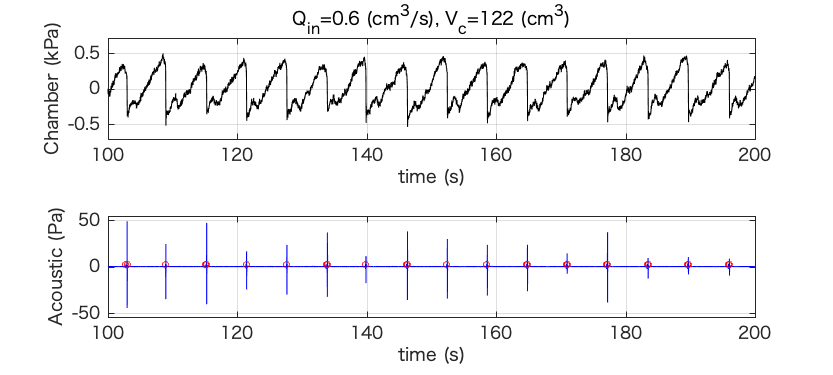
\includegraphics[scale=1] {MonoPAtime.png} 
\caption{Chamber pressure and acoustic wave (Unimodal STW). Upper: Chamber pressure, Lower: Acoustic wave. Red markers represent the triggered time of abrupt pressure drop.}
\label{MonoPAtime}
\end{center}
\end{figure} 

\begin{figure}[H]
\begin{center}
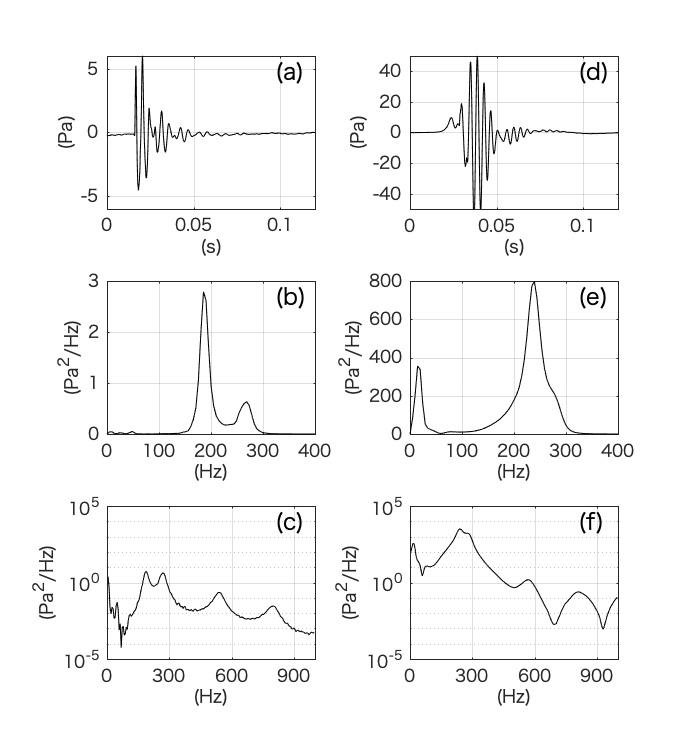
\includegraphics[scale=1] {Monowaveform.png} 
\caption{Representative acoustic waveform and its spectrum: Unimodal STW. (a) the high-frequency pulse (b, c). (d) the low-frequency pulse (e, f).}
\label{Monowaveform}
\end{center}
\end{figure}

\begin{figure}[H]
\begin{center}
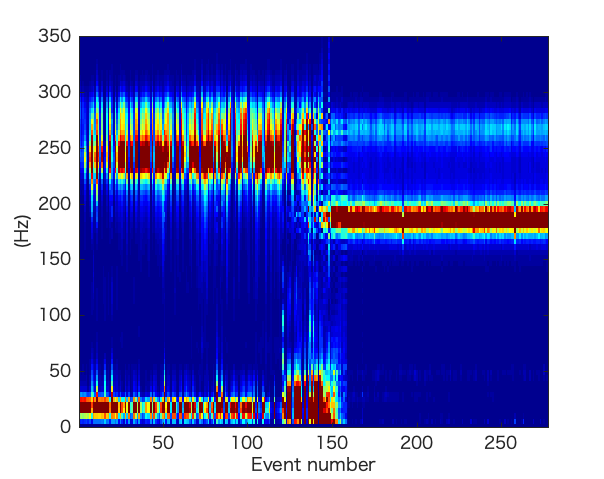
\includegraphics[scale=1] {Monopspec.png} 
\caption{An event-spectrum representation (Unimodal STW): Pulses were triggered that the maximum amplitude of the pulse was greater than 1 Pa, regardless of whether the pressure abruptly decreased or not.
The vertical axis shows the frequency and the horizontal axis shows the pulse event, sort by the peak at the 20 Hz.}
\label{Monopspec}
\end{center}
\end{figure} 

\begin{figure}[H]
\begin{center}
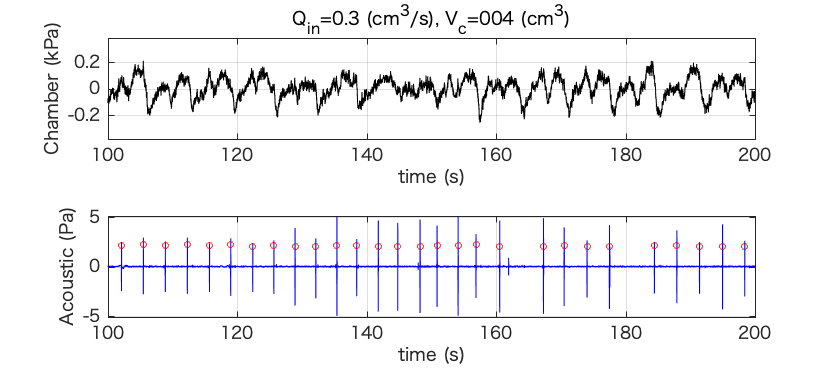
\includegraphics[scale=1] {FlctPAtime.png} 
\caption{Chamber pressure and acoustic wave: Small fluctuation, refer to Fig. \ref{MonoPAtime}}
\label{FlctPAtime}
\end{center}
\end{figure} 

\begin{figure}[H]
\begin{center}
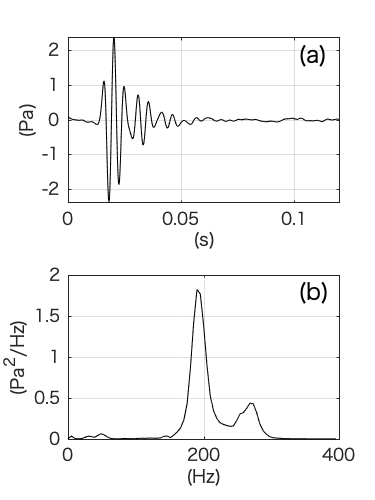
\includegraphics[scale=1] {Flctwaveform.png} 
\caption{Representative acoustic waveform and its spectrum: Small fluctuation}
\label{Flctwaveform}
\end{center}
\end{figure} 

\begin{figure}[H]
\begin{center}
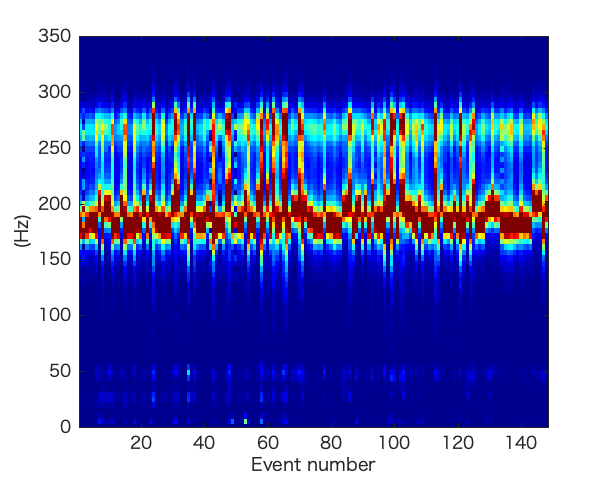
\includegraphics[scale=1] {Flctpspec.png} 
\caption{An event-spectrum representation: Small fluctuation, refer to Fig. \ref{Monopspec}}
\label{Flctpspec}
\end{center}
\end{figure} 

\begin{figure}[H]
\begin{center}
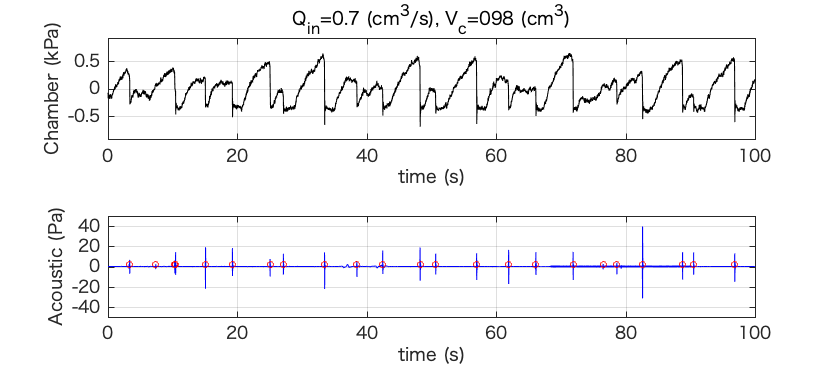
\includegraphics[scale=1] {DistPAtime.png} 
\caption{Chamber pressure and acoustic wave: Disturbed STW, refer to Fig. \ref{MonoPAtime}}
\label{DistPAtime}
\end{center}
\end{figure} 

\begin{landscape}
\begin{figure}[H]
\begin{center}
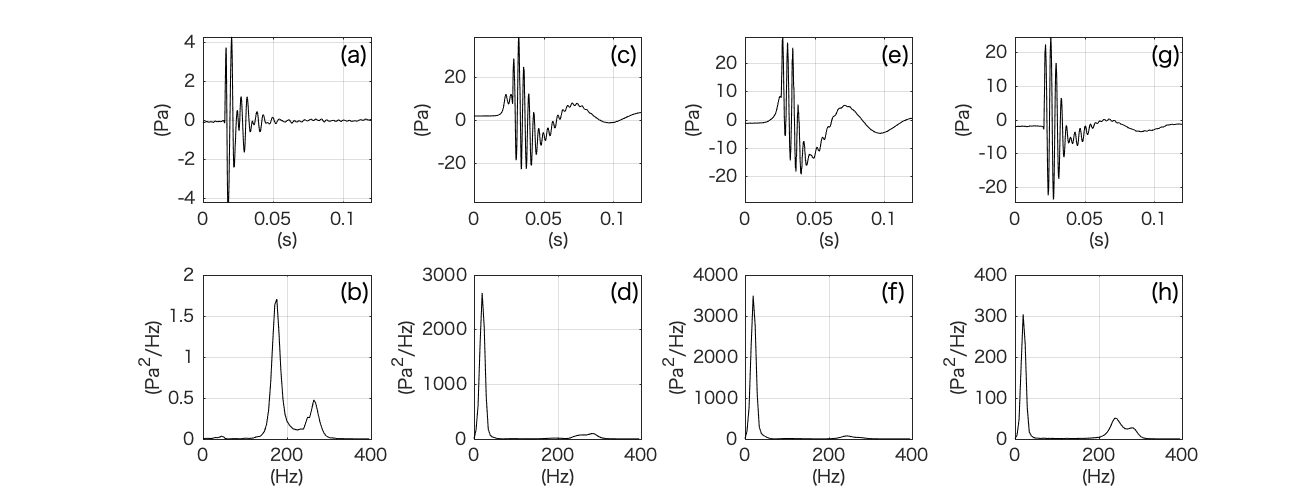
\includegraphics[scale=1] {Distwaveform.png} 
\caption{Representative acoustic waveform and its spectrum: Disturbed STW 発生時の代表的波形; (a, b) the high-frequency pulse, (c-h) the low-frequency pluse; (c, d) Type 1; (e, f) Type 2; (g, h) Type 3}
\label{Distwaveform}
\end{center}
\end{figure} 
\end{landscape}


\begin{figure}[H]
\begin{center}
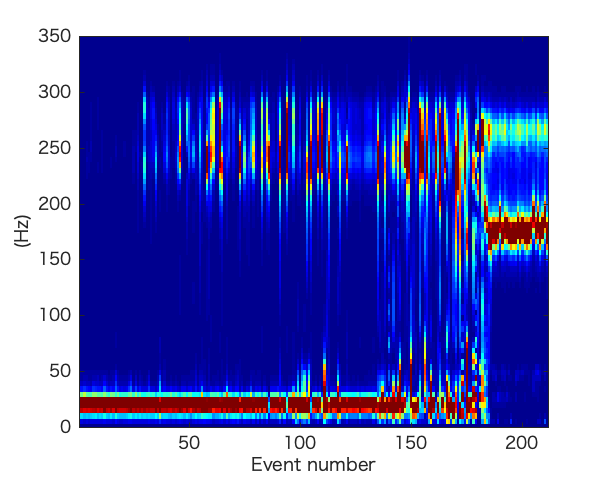
\includegraphics[scale=1] {Distpspec.png} 
\caption{An event-spectrum representation: Disturbed STW, Fig. \ref{Monopspec}のキャプションを参照}
\label{Distpspec}
\end{center}
\end{figure} 

\begin{figure}[H]
\begin{center}
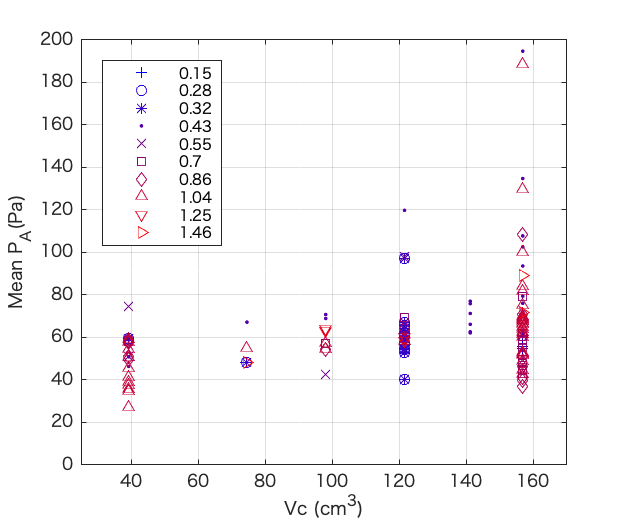
\includegraphics[scale=1] {QVA.png} 
\caption{Experimental parameters ($V_\mathrm{c}$, $Q_\mathrm{in}$) and mean amplitude of acoustic pulse: Makers represent $Q_\mathrm{in}$. The unit of legend is cm$^3$/s.}
\label{QVA}
\end{center}
\end{figure} 

\begin{landscape}
\begin{figure}[H]
\begin{center}
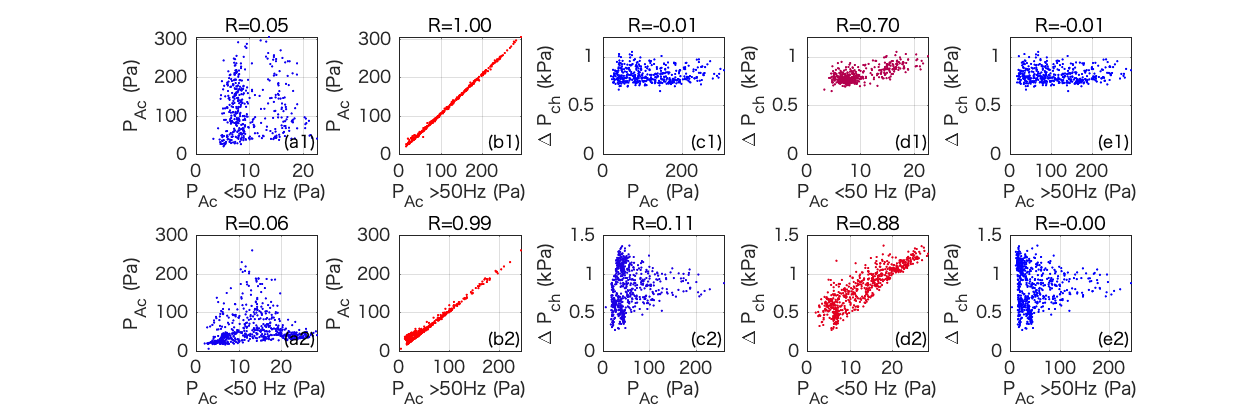
\includegraphics[scale=1] {PAPCall.png} 
\caption{Comparison of the amplitude of the acoustic pulse and chamber pressure: a1 - e1 shows the results under the Unimodal STW and a2 - e2 for the Disturbed STW.
Acoustic pulses correspond to the abrupt pressure drop in the chamber pressure.
R is the correlation coefficient of each parameter. 
(a, b) The raw amplitude of acoustic pulses $P_{AC}$, and amplitude of low-frequency band ( < 50 Hz, a), and high-frequency band (> 50 Hz, b).
(c, d, e) The amplitude of pressure changes ($\Delta P_{ch}$), and $P_{AC}$ (c), low-frequency band (< 50 Hz, d), high-frequency band (> 50 Hz, e).}
\label{PAPCall}
\end{center}
\end{figure} 
\end{landscape}



\clearpage
\subsubsection{Comparison with flow in the pipe}
実験で撮影したパイプ内流れ映像, チャンバー圧力変化と, 空気振動パルスの発生を比較する.

STWが発生している時, Fig. \ref{ImPenlarged}によれば, チャンバー圧力の急減圧, すなわち, スラグ-環状流遷移が発生する際の液スラグ膜破裂にともなって, 振幅の大きな (> 10 Pa) 空気振動パルスが発生している. 
この時の波形は Fig. \ref{Monowaveform}d で示した, 低周波パルスである. 
低周波パルス発生直後は, パイプ上端からチャンバーまでガス相が一続きになっている.
空気振動波形低周波帯 (< 50 Hz) に, ローパスフィルターをかけた波形と, チャンバー圧力波形を比較する (Fig. \ref{ImPenlarged}). 
空気振動低周波帯の波形は, チャンバー圧力減圧時の波形と対応しており, 空気振動低周波帯の増減圧にかかる時間 ($\sim$ 0.05 s) は, チャンバー圧力の減圧にかかる時間と同程度である.

The acoustic pulses were compared with the chamber pressure change and the flow in the pipe taken in the experiment.

According to Fig. \ref{ImPenlarged}, when the STW was measured, with the abrupt chamber pressure drop, that is, the rupture of the liquid slug membrane when slug-to-annular flow transition occurred, acoustic pulses with large amplitude (>10 Pa) were measured.
These waveforms were the low-frequency pulse indicated by Fig. \ref{Monowaveform}d.
Immediately after the low-frequency pulse, the gas phase was continuous from the upper end of the pipe to the chamber.
The low pass filtered acoustic waveform and the chamber pressure waveform were compared (Fig. \ref{ImPenlarged}).
The acoustic waveform in the low-frequency band corresponded to the chamber pressure waveform at the abrupt pressure drop.
The time required for increasing and decreasing the low-frequency band of the acoustic waveform was about the same as the time required for depressurizing the chamber pressure.

また, チャンバー圧力の急減圧の直前に, Precursor的に, 小さな空振パルスが発生している. 
この時の小さなパルスは, 全ての液スラグが破裂する直前の, 最上端液スラグ膜破裂に対応しており, Fig. \ref{Monowaveform}a で示した高周波パルスに対応している. この高周波パルスが発生するとき, まだパイプの中にはスラグ流れが存在している. 

Just before the abrupt pressure drop of the chamber pressure, a small acoustic pulse was generated as a precursor.
The small pulses corresponded to the rupture of the uppermost liquid slug membrane immediately before all the liquid slug ruptures, corresponding to the high-frequency pulses shown in Fig. \ref{Monowaveform}a.
When these high-frequency pulses were generated, slug flow still existed in the pipe.

Small fluctuation発生時, 準定常的的スラグ流のうち, 最も上端の液スラグ膜が破裂する際に空気振動が発生している. この時, 前章で記述したように, 一番上の膜が破裂しても, 後に続く液スラグ膜は破裂せずそのまま上昇を続けることから, 発生時の状況は, STWにおけるPrecursor的高周波パルスと同じである.

Under the small fluctuation conditions, the acoustic pulse occurred when the uppermost liquid slug membrane ruptured in quasi-steady slug flow. 
At this time, as described in the previous, even if the uppermost liquid slug membrane ruptured, the subsequent liquid slug membrane would not rupture and continue to rise as it is, so the situation was the same as the precursor high-frequency pulse under STW conditions.

Disturbed STW発生時には, Unimodal STW発生時に比べて, 空気振動波形にバリエーションがある (Fig. \ref{Distwaveform}). 
そこで, パイプ内流れを高速度撮影 (8000 frame/s) で撮影することで, スラグ-環状流遷移時の液スラグ破裂過程と, 空気振動波形の対応を検討する.

When the disturbed STW occurred, there were variations in the acoustic waveform (Fig. \ Ref {Distwaveform}) compared to when the unimodal STW occurred.
Therefore, by taking the flow in the pipe at high-speed movies (8000 frames/s), the correspondence of the process of rupture of liquid slug membrane and the acoustic waveform at the slug-to-annular flow transition was investigated.

Fig. \ref{Distwaveform}c のような波形 (Type 1) が発生するときのパイプ内流れと空気振動波形の様子を Fig. \ref{Type1} に示す. 
この波形はUnimodal STWの際に発生する低周波パルス (Fig. \ref{Monowaveform}d) とよく似た波形であり, 高周波と低周波の振動がほぼ同時に始まる. 
このとき, パイプには液スラグが3つ発生しており, 便宜上, 上からスラグ1, 2, 3とする. 
この例では, スラグ1が破れた $t=1210$ msに, Precursor的高周波パルスが発生した. 
次に, スラグ2と3が 10 ms程度の時間差で破裂したが, その時に高周波と低周波を含む振動が発生したことがわかった.

Fig. \ref{Type1} shows the flow in the pipe and the acoustic waveform when a waveform (Type 1) like Fig. \ref {Distwaveform}c occurred.
This waveform was similar to the low-frequency pulse (Fig. \ref {Monowaveform}d) generated in the case of the Unimodal STW, and the high frequency and low-frequency oscillation started almost at the same time.
At this time, three liquid slugs were generated in the pipe, and for convenience sake, they are assumed to be slug 1, 2, and 3 from above.
In this example, a precursor high-frequency pulse was generated at $t = 1210$ ms when slug 1 ruptured.
Slugs 2 and 3 subsequently ruptured with a time difference of about 10 ms, and acoustic wave including high frequency and low frequency occurred at that time.

Fig. \ref{Distwaveform}e のような波形 (Type 2) が発生するときのパイプ内流れと空気振動波形の様子を Fig. \ref{Type2} に示す. 
波形は緩やかに立ち上がり, そのままピークに達し, その後高周波の振動が発生する. 
このような特徴は Unimodal STW発生時にはほとんど見られず, Disturbed STWに特徴的な波形であった. 
Fig. \ref{Type2} の例では, 液スラグが3つ発生しており, 上からスラグ1, 2, 3とする. スラグ1と3は $t=1650$ msにほぼ同時に破裂するが, この時, まだスラグ2は膜状になるほど薄くなっていない. スラグ1, 3の破裂をきっかけに, スラグ2の上昇速度は大きくなっていき, $t=1720$ ms に破裂する. 破裂前の液膜の変形は, Fig. \ref{Type1} と比べて大きいことから, 緩やかな空気振動の立ち上がりは, スラグ2の破裂直前の変形によるものであると考えられる.

Fig. \ref{Type2} shows the flow in the pipe and the acoustic waveform when a waveform (Type 1) like Fig. \ref {Distwaveform}e occurred.
The waveform gradually raised, it reached its peak as it was, and then the high-frequency pulse was generated.
Such features were rarely seen when Unimodal STW occurred and were distinctive waveforms under Disturbed STW conditions.
At this time, three liquid slugs are generated in the pipe, and for convenience sake, they are assumed to be slug 1, 2, and 3 from above.
Slugs 1 and 3 ruptured at about the same time at $ t = 1650 $ ms, but at this time, the slug 2 was not thin enough to become membrane.
After the rupture of the slugs 1 and 3, the rising speed of the slug 2 increased and ruptured at $ t = 1720 $ ms.
Since the deformation of the liquid membrane just before rupture was larger than Fig. \ref {Type 1}, it is considered that the gentle acoustic pressure rise was due to the deformation just before the rupture of the slug 2.

Fig. \ref{Distwaveform}g のような波形 (Type 3) が発生するときのパイプ内流れと空気振動波形の様子を Fig. \ref{Type3} に示す. 空気振動波形は, 液スラグの破裂の直前に, わずかに周期のやや長い増減圧がある. 
液スラグ破裂と同時に鋭い立ち上がりに続いて, 高周波振動が始まり, その後低周波振動が続く. 
パイプ内流れは, パイプ下端で発生した液スラグが, 次の液スラグ再生成の前に液膜流内で破裂している. 
高周波パルス (Fig. \ref{Distwaveform}a) と波形が似ているが, この場合, 液スラグ破裂はスラグ-環状流遷移に対応するために, 低周波の振動も発生している.

Fig. \ref{Type3} shows the flow in the pipe and the acoustic waveform when a waveform (Type 1) like Fig. \ref {Distwaveform}g occurred. 
The acoustic waveform had a longer period fluctuation, just before the rupture of the liquid slug.
At the same time as rupture of liquid slug membrane, there is a sharp rise of acoustic pressure, followed by high-frequency oscillation, then low-frequency oscillation. 
In the pipe flow, the liquid slug generated at the bottom of the pipe ruptured in the downward film flow before the next liquid slug reconstruction.
It was similar to the high-frequency pulse (Fig. \ref{Distwaveform}a), but in this case, the liquid slug rupture also generated the low-frequency pulse to correspond to the slug-to-annular flow transition.

\clearpage
\subsubsection{Relationship between acoustic pulse amplitude and chamber pressure amplitude}\label{AcoChp}
Unimodal STW, Disturbed STW 発生時の空気振動とチャンバー圧力の関係を Fig. \ref{PAPCall} に示す. 
空気振動パルスは, スラグ-環状流遷移発生にともなう低周波パルスの振幅と比較する. 
チャンバー圧力振幅と空振生波形振幅は全く相関がない (Fig. \ref{PAPCall}c). 
これは, Fig. \ref{MonoPAtime} において, Unimodal STW 発生時にチャンバー圧力が毎サイクルほぼ一定であるにもかかわらず, 空気振動パルスの振幅が一定でないことからもわかる. 
低周波パルスは, 低周波帯と (<50 Hz) と高周波帯 (> 50 Hz) にピークを持つことから, それぞれの帯域でローパス, ハイパスフィルターをかけた波形の振幅と, チャンバー圧力を比較する (Fig. \ref{PAPCall}d, e). 
低周波パルスの低周波帯ピークとチャンバー圧力に強い相関がある (Fig. \ref{PAPCall}d). 
Fig. \ref{PAPCall}d1 では チャンバー圧力振幅がほぼ一定であるため, 関係がやや不明瞭であるが, Fig. \ref{PAPCall}d2 ではチャンバー圧力振幅と空気振動低周波帯の振幅に強い相関があることがわかる.

Fig. \ref{PAPCall} shows the relationship between acoustic pulse and chamber pressure amplitude when Unimodal STW and Disturbed STW were measured.
The acoustic pulses are compared with the amplitude of the low-frequency pulse associated with slug-to-annular flow transition occurrence.
There is no correlation between the chamber pressure amplitude and the raw acoustic waveform amplitude at all (Fig. \ref {PAPCall}c).
This is also evident from Fig. \ref{MonoPAtime}, even though the chamber pressure amplitude were almost constant every cycle when Unimodal STW occurs, the amplitude of the acoustic pulses were not constant.
There was a strong correlation between the low-frequency band peak of the low-frequency pulse and the chamber pressure (Fig. \ref {PAPCall}d).
In Fig. \ref {PAPCall}d1 the relationship is somewhat obscure because the chamber pressure amplitude is nearly constant.
There is a strong correlation between the chamber pressure amplitude and the amplitude of the low-frequency band of the acoustic pulse in Fig. \ref {PAPCall}d2.

\clearpage
\subsection{Discussion}\label{ACOdisc}
\subsubsection{The acoustic spectrum}
実験に見られる空気振動は, 低周波パルスと高周波パルスに大別されることが分かった. 
管内における膜の破裂によって励起される特徴的な周波数がパイプ内の気柱共鳴である可能性を検討する. 
パイプ内の膜破裂による空気振動に着目した先行研究 \citep{Vidal2006a, Sanchez2014} では, 特徴的な周波数は閉管の気柱共鳴で説明できるとしていた. 
本実験では, パイプの下端はチャンバー側に解放されており, 上端は解放されているため, パイプの構造は両端開口 (開管) になっている. 
開管の気柱共鳴の $n$倍振動 ($n=1,2,3...$)の周波数 $f^{op}_{n}$はパイプ長さ $L$, 音速 $c_{air}$を用いて, 以下のように与えられる:
\begin{eqnarray}
f^{op}_{n}=\frac{n}{2L} c_{air}
\end{eqnarray}

It is found that the acoustic pulse observed in the experiment is divided into the low-frequency pulse and the high-frequency pulse.
We investigate the possibility that the characteristic frequency excited by the rupture of the membrane inside the pipe is the air column resonance in the pipe.
Previous studies focusing on acoustic wave due to membrane rupture in pipes \citep{Vidal 2006a, Sanchez2014} assumed that the characteristic frequencies could be explained by closed air column resonance.
In this experiment, since the lower end of the pipe is released to the chamber side and the upper end is released to the atmosphere, the structure of the pipe is open at both ends (open pipe).
The frequency $ f^{op}_{n}$ ($ n = 1, 2, 3 ... $) of the air column resonance of the open pipe with the length $L$ is given as follows under the sound speed $c_{air}$:

高周波パルス発生時には, パイプの途中に液スラグが存在し, 上端のみが開口する, 閉管となっている. 
閉管の気柱共鳴の $2n-1$倍振動 ($n=1,2,3...$) 周波数 $f^{cl}_{2n-1}$ は, 閉管部分のパイプ長さ $L_1$として, 
\begin{eqnarray}
f^{cl}_{2n-1}=\frac{2n-1}{4L_1} c_{air}
\end{eqnarray}
と与えられる.

At the time of generation of the high-frequency pulse, there is a closed air column where a liquid slug exists in the middle of the pipe and only the upper end opens.
The frequency $f^{cl}_{2n-1}$ of the closed air column of which length of $L_1$ is given as:

低周波パルスの発生時, パイプの中は連続したガス流れになっていることから, パイプが開管になっている.
また, 低周波パルスの低周波帯の増減圧にかかる時間は, チャンバー急減圧にかかる時間と同程度であった (Fig. \ref{ImPenlarged}). 
これは, 空気振動低周波帯のシグナルが, チャンバーからのガスの放出によって励起されている可能生を示唆している. 
そこで, 特徴的な周波数ピークを作る要因として, チャンバー内のガスがバネの役割を果たすパイプ-チャンバー内全体の共鳴, すなわち, ヘルムホルツ共鳴が考えられる.

When low-frequency pulses are measured, the pipe has open ends because they are continuous gas flow in the pipe.
Moreover, the time required for the low-frequency pulse was about the same as the time needed for the abrupt pressure drop of the chamber (Fig. \ref{ImPenlarged}).
This suggests that the signal of the acoustic low-frequency band was excited by the emission of gas from the chamber.
Therefore, as a factor of generating characteristic frequency peaks, the resonance of the entire pipe-chamber, that is, Helmholtz resonance, in which gas in the chamber and pipe plays a role of a spring can be considered.

ヘルムホルツ共鳴によって励起される周波数 $f_h$は, パイプの断面積 $S$ とした時, チャンバー体積 $V_\mathrm{c}$ を用いて,  
\begin{eqnarray}
f_{h}=\frac{c_{air}}{4\pi} \sqrt{  \frac{S}{V_\mathrm{c} L }   } \label{Helmeq}
\end{eqnarray}
と与えられる. 

The frequency excited by the Helmholtz resonance ($f_h$) is expressed as follows using the chamber volume $V_\mathrm{c}$ when the sectional area of ​​the pipe is $S$:

Fig. \ref{Helm}に, パイプ全長 630 mm, パイプ内径 2.5 (1.8) mm, 音速 340 m/sとした時の, ヘルムホルツ共鳴および気柱共鳴によって励起される基本周波数を示す. 

Fig. \ref{Helm} shows the calculated fundamental frequency excited by Helmholtz resonance and air column resonance when the pipe length is 630 mm, the inner pipe radius is 2.5 (1.8) mm, and the sound speed is 340 m/s.

低周波パルスにおいて, 発生する低周波ピークは, パイプ半径が 1.8 mm の時のヘルムホルツ共鳴の周波数ピークとほぼ一致している. 
装置のパイプ半径は 2.5 mm であるが, 液膜流が存在しているため, 実効的なガス流路半径が小さくなっていると考えられる. 

In the low-frequency pulse, the generated low-frequency peak almost coincides with the frequency peak of the Helmholtz resonance when the pipe radius is 1.8 mm.
The actual pipe inner radius is 2.5 mm, but since the downward liquid film flow is present, it is considered that the effective gas flow path radius is small.

また, 低周波パルスは高周波帯 (230 - 270 Hz) にもピークを持っていた. 
これは, 630 - 700 mm の開管パイプの気柱共鳴基本周波数に相当し, 実験パイプの全長 630 mmと整合的である. 

Besides, the low-frequency pulse had a peak also in the high-frequency band (230 - 270 Hz).
This corresponds to the air column resonance fundamental frequency of an open pipe of 630 - 700 mm, consistent with the total length of 630 mm of the experiment pipe.

高周波パルスのピークはやや低い周波数で, 180 - 200 Hz 付近にピークを持っていた. 
これは, 430 - 460 mm の閉管パイプの基本周波数に相当するが, 液スラグはパイプ下端から 200 mm 程度のところで破裂するという実験での観察結果と整合的な値である. 

The peak of the high-frequency pulse was a slightly lower frequency and had a peak around 180 - 200 Hz.
This corresponds to the fundamental frequency of a closed pipe of 430 - 460 mm, and liquid slug rupturing at about 200 mm from the lower end of the pipe is consistent with the observation result in the experiment.

以上の考察から, 実験にみられる空気振動は, 低周波帯と高周波帯にピークを持っており, 低周波帯はパイプ-チャンバー全体の構造を反映したヘルムホルツ共鳴, 高周波帯はパイプの構造を反映した気柱共鳴の基本周波数によって説明できると考えられる.

From the above discussion, it can be considered that the air vibrations seen in the experiment can be explained by the fundamental frequency of the air column resonance reflecting the pipe structure in the high-frequency band and the Helmholtz resonance reflecting the structure of the entire pipe-chamber in the low-frequency band.

\subsubsection{Characteristic acoustic waveform}
Unimodal STWと, Disturbed STWでは, スラグ-環状流遷移発生にともなう低周波パルスの波形の特徴が異なっていた. 
これは, \S \ref{preflowanalysis}でも指摘したように, Disturbed STWにおける液膜流厚み及び液スラグ上昇速度のばらつきに起因していると考えられる. これについて, 考察を進める.

Under the Unimodal STW and the Disturbed STW conditions, the characteristics of the waveform of the low-frequency pulse were different.
This is thought to be due to the disturbances of the downward film flow thickness and the liquid slug rising speed in Disturbed STW.

Unimodal STWが発生しているとき, 液膜流の厚みにはほとんどばらつきがなかった (Fig. \ref{RDKhist}). 
このため, 液スラグの上昇の仕方も各STWサイクルでほとんど変わらない. 
高周波パルスは最上部の液スラグだけが先行して破裂することによって発生しており, Fig. \ref{Monopspec} によれば, 高周波パルスと低周波パルスはほぼ同数であった. 
このことから, Unimodal STWでは, スラグ-環状流遷移過程も毎サイクルほとんど変わらず, 毎回最上部の液スラグが先行して割れて高周波パルスを発生し, それに続いてパイプ内の液スラグがほぼ一斉に (10 ms以内) に破裂して低周波パルスを発生していると考えられる.

When Unimodal STW was measured, the thickness of the downward film flow had almost no variation (Fig. \ref{RDKhist}).
For this reason, the ascending speed of the liquid slug hardly changed in each STW cycle.
According to Fig. \ref{Monopspec}, the high-frequency and the low-frequency pulse were almost the same.
From these results, under the Unimodal STW conditions, the slug-to-annular flow transition process also hardly changes every cycle, with the top liquid slug preceding and breaking each time to generate high-frequency pulses, followed by rupturing almost all of the liquid slug to generate the low-frequency pulse.

Disturbed STWでは, 液膜流途中で液スラグ再生成が発生することによって, 液スラグの上昇速度にばらつきが生じ, 結果として液膜流厚みにもばらつきが生じていた (Fig. \ref{RDKhist}). 
このことで, スラグ-環状流遷移時の液スラグ膜破裂過程もばらつき, 様々な空気振動波形が計測されていると考えられる. 
Fig. \ref{Distpspec} によれば, Unimodal STW発生時に比べて, Disturbed STWでは, 高周波パルスの割合が少ない. 
これは, スラグ-環状流遷移の際に, 複数液スラグのうち, 必ずしも最上部の液スラグから割れ始めるのではなく, 下部の液スラグから破裂する, または, 複数の液スラグが再生成する前に液スラグが破裂するといった異なるスラグ-環状流遷移過程も含んでいることを反映している.
特に, Fig. \ref{Type2} の空気振動波形に対応する破裂直前に, 液スラグ急速に加速するような時には, それだけ多くの液を液膜流に排出し, 大きな液膜流表面擾乱を発生させると考えられる. 大きな液膜流表面擾乱が発生すれば, 液膜流途中での液スラグ再生成が発生しやすくなり, Disturbed STWのような周期の乱れを生み出すと考えられる (\S \ref{precond}). 

Under the Disturbed STW conditions, the reconstruction of the liquid slug in the middle of the downward film flow caused variations in the rising speed of the liquid slug, and as a result, the downward film flow thickness also varied (Fig. \ref{RDKhist}).
As a result, the process of rupture of the liquid slug membrane at the slug-to-annular flow transition also varies, and various acoustic waveforms are considered to be measured.
According to Fig. \ref{Distpspec}, under the Disturbed STW conditions, the ratio of the high-frequency pulses is smaller than when Unimodal STW occurs.
This is because, at the time of slug-to-annular flow transition, rather than starting to rupture from the uppermost liquid slug, it bursts from the liquid slug at the lower part.
It also reflects the different slug-to-annular flow transition process, such as liquid slug bursting before multiple liquid slugs reconstruction.
In particular, when the liquid slug rapidly accelerates immediately before the rupture corresponding to the acoustic waveform of Fig. \ref{Type2}, a large amount of liquid is discharged into the downward film flow so that a large liquid film flow surface disturbance left behind.
If a large surface disturbance of downward film flow occurs, liquid slug reconstructions are likely to occur in the middle of the downward film flow, which is considered to produce a periodic disturbance like Disturbed STW.

\subsubsection{空振各帯域振幅, チャンバー圧力振幅の関係}
空気振動波形のうち, ヘルムホルツ共鳴に起因する低周波帯空気振動の振幅は, チャンバー圧力振幅と良い相関を示した. 
Fig. \ref{AcoAmVP} では, STWが発生するすべての実験条件において, 空気振動低周波帯の振幅 (縦軸) と, チャンバー圧力振幅, チャンバー圧力振幅とチャンバー体積の積 (噴出ガス量に相当) を比較した結果である. 
この結果によれば, 空気振動低周波帯の振幅は, チャンバーの圧力振幅, すなわちスラグ-環状流遷移直前のチャンバー過剰圧と良い比例関係にある. 
一方で, チャンバーの体積 ($V_\mathrm{c}$) の情報がなければ, 噴出ガス量の推定ができないことも示している. 

The amplitude of low-frequency band acoustic waveform due to Helmholtz resonance showed a good correlation with chamber pressure amplitude.
Fig. \ref{AcoAmVP} shows the results of comparison between the amplitude of the acoustic low-frequency band (vertical axis), the chamber pressure amplitude, the product of the chamber pressure amplitude and the chamber volume equivalent to the amount of ejected gas.
According to this result, the amplitude of the acoustic low-frequency band has a good proportional relationship with the pressure amplitude of the chamber, that is, the chamber overpressure just before the slug-to-annular flow transition.
On the other hand, if there is no information on the volume of the chamber, it can be inferred that it is hard to estimate the amount of the ejected gas.

Eq. (\ref{Helmeq}) によれば, パイプの構造 ($S$, $L$) と音速が既知でない限り, 低周波帯のピーク周波数  ($f_{h}$)  から $V_\mathrm{c}$ を見積もることも難しい. 
一方で, 音速さえ既知であれば, 低周波パルスに含まれる高周波帯のピーク周波数 ($f^{cl}_{1}$) から, $L$ を推定することができる.
 例えば, パイプの中が見えない場合でも, $S$ の値として, 表面で観察できるパイプ上端のガス流路断面積を用いれば, Eq. (\ref{Helmeq}) を用いて $V_\mathrm{c}$ を推定できる. 
ただし, 実験の結果 (Fig. \ref{Helm})によれば, $S$ の値として液膜流の存在よって実際のパイプ断面積よりも小さいガス流路断面積を用いた方が, 実験パラメータ $V_\mathrm{c}$ をより説明することができた. すなわち, $S$ の値としてパイプの断面をそのまま用いると, チャンバー体積を過大評価してしまう可能性には注意が必要である.

According to Eq. (\ref{Helmeq}), unless the pipe structure ($S$, $L$) and the speed of sound are known, it is also difficult to estimate $V_\mathrm{c}$ from the peak frequency ($f_{h}$) of the low-frequency band.
On the other hand, if even the sound speed is known, $L$ can be estimated from the peak frequency of the high-frequency band ($f^{cl}_{1}$) included in the low-frequency pulse.
Careful attention should be paid to the possibility of overestimating the chamber volume if the cross-section of the pipe was used as the value of $S$ as it was.

\clearpage
\subsubsection{Implication for volcano}\label{acoshisa}
実験の結果からは, 空気振動波形の違いによるチャンバー圧力振動周期への影響を定量的には議論できなかったが, チャンバー圧力振動周期が乱れるような時に, 空気振動波形にバリエーションがある, ということを実験の解析から示した.
Disturbed STW発生時に見られた, Fig. \ref{Type2} の空振波形では, 高周波振動に先行して, 緩やかな波形の立ち上がりが見られた. 
このような先行相は, ブルカノ式噴火にともなった観測例が報告されている.
 \cite{Yokoo2009}では, 空振波形とビデオ映像を合わせて, 爆発の主要相に先行する空振記録の緩やかな増圧は, 爆発直前の火口直下ガスポケットの膨張による, 浅部プラグの変形に起因していると推定している. 
実験の結果を基にすれば, このようなプラグの破壊にともなう火口浅部構造の変化や, 噴出物の再堆積等が, 噴火の周期に影響を及ぼしているかもしれない (\S \ref{sugvolc}). 

From the results of the experiment, we could not quantitatively discuss the influence of the difference in the acoustic waveform on the disturbance of chamber pressure cycle.
On the other hand, the experimental analysis showed that there were variations in the acoustic waveform when the chamber pressure cycle was disturbed.
In the acoustic waveform of Fig. \ref{Type2} when Disturbed STW occurred, a gentle rise of the acoustic pressure was observed before the high-frequency signal.
Observation examples accompanying the Vulcanian eruption have been reported for such a preceding phase.
Based on the infrasound record and the video image, it was presumed that the gradual pressure increase of the infrasound record preceding the main phase of the explosion was caused by the deformation of the shallow plug due to the expansion of the gas pocket immediately before the explosion \citep{Yokoo2009}.
Based on the results of experiments, changes in the shallow vent structure and redeposition of the ejecta due to the destruction of such a plug may affect the cycle of the eruption.

もう一つ, この実験から得られた重要な知見は, 空振のある特徴に着目すれば, 地下の圧力源圧力変化にともなう地盤変動といった地下の情報を含んでいる可能性がある, という点にある.
実験では, 空振低周波帯のシグナルと, チャンバー減圧が同程度のタイムスケールであり (Fig. \ref{ImPenlarged}), このタイムスケールに相当する低周波帯の空気振動振幅と, チャンバー圧力振幅に対応関係があった. 
この結果を踏まえると, 実際の観測においても, 地盤変動と同程度のタイムスケールの空振シグナルに着目すれば, 地盤変動と空振の対応関係を見い出すことができるのではないかと考える.
先行研究において, 火山活動にともなって発生する空振と噴出量や噴出率の関係は様々なメカニズムが提案されており, 統一的な理解は進んでいないが, 特定のメカニズムに着目すれば, 噴出量・噴出率といった情報との対応関係を見いだせる可能性があると指摘されている \citep{Ichihara2016a}.

Another important suggestion obtained from this experiment is that some features of the infrasound signal may contain underground information such as ground deformation due to underground pressure source change.
In the experiment, the signal of the low-frequency band and the chamber pressure drop were on the same time scale, and there was a correspondence relationship between both amplitudes.
Given this result, we also consider that in the actual observation, if we focus on the time-scale infrasound signals of the same as the ground deformation, there is a possibility to find the correspondence relationship between the ground deformation and the infrasound signal.
In the previous study, various mechanisms have been proposed for the relationship between infrasound and the amount of eruption mass and/or rate, and unified understanding has not progressed.
Focusing on specific mechanisms of infrasound, it is pointed out that there is a possibility of finding correspondence with information such as eruption mass and/or rate \citep{Ichihara2016a}.

実験では特定の周波数ピークを含む空気振動周波数帯の振幅と, チャンバー圧力振幅を比較した. 
火山噴火にともなう空振にも, 特徴的な周波数ピークがあることが先行研究で報告されている \citep{yokoo2012bo}. 
実験との対比として, 火山活動にともなって発生する空振において, ある特定の周波数帯が, 地盤変動といった地下の情報との対応関係を検討する必要があると考える.

In the experiment, the amplitude of the acoustic frequency band including the specific frequency peak was compared with the chamber pressure amplitude.
Previous studies have reported that there are several characteristic frequency peaks in the infrasound signal accompanying volcanic eruption \citep{yokoo2012bo}.
As a comparison with the experiment, it is necessary to consider the correspondence relation between the specific frequency band of the infrasound signal and the underground information such as the ground deformation.

先行研究では, 爆発にともなうパルス状の空振波形に着目し, 積算体積を推定する手法が提案されており \citep{Johnson2003}, 例えば, 桜島昭和火口活動にともなった空振記録と, 火山灰噴出量との比較が試みられている \citep{Fee2017a}. 
しかし一方で, 例えば桜島における爆発的噴火にともなう地盤変動の継続時間は, 数分から数十分であり \citep{Iguchi2012, Iguchi2013a}, 爆発パルスの継続時間は数十秒である.
\cite{DelleDonne2016} では, Ash-richな噴火においては, 爆発の初動パルスだけではなく, 後続相にも注目することで, 噴火にともなって放出される熱エネルギーと良い相関が得られること指摘している. 
本実験の結果を踏まえれば, パルス的な空振だけに注目するのではなく, 継続時間の長い後続相にまで着目することで, 地盤変動に対応するような地下の情報を含んでいる可能性があることが本実験から示唆されると考えられる.

In the previous research, a method to estimate the accumulated volume by paying attention to the pulsed infrasound waveform accompanying the explosion has been proposed \citep{Johnson2003}.
For example, attempts have been made to compare the infrasound records accompanying the Sakurajima Showa crater activity with volcanic ash ejection volume \citep{Fee2017a}.
However, while the duration of the explosion pulse is several tens of seconds, the duration of the ground deformation accompanying the explosive eruption on Sakurajima, for example, is several minutes \citep{Iguchi2012, Iguchi2013a}.
\cite{DelleDonne2016} pointed out that not only the initial pulses of the explosion but also the subsequent phases are considered for the analysis so that to a good correlation is obtained between infrasound-derived volume and the thermal energy with the eruption.
Based on the results of this experiment, It is suggested from this experiment that focusing not only on the initial phase of infrasound but also on subsequent phases may obtain underground information that corresponds to ground deformation.


%bibliography作成にはMendeleyを用いた
%Mendeleyを用いてbibファイルをこのtexファイルと同じディレクトリ内に作成. ターミナル上で " pbibtex ファイル名" を実行してコンパイル
%http://pioneerboy.hatenablog.com/entry/2014/01/18/214446
%http://ftp.yz.yamagata-u.ac.jp/pub/CTAN/macros/latex/contrib/natbib/natbib.pdf
%Agu08.bst をどこから入手したのかわすれてしまった...
%agu_template内
\clearpage \newpage
\bibliographystyle{agu08}
\bibliography{library} 
\addcontentsline{toc}{section}{References}


\end{document}